\documentclass{article} 

\graphicspath{{/home/david/Book/Chapters/2.Vectors/VectorOperations/pic/}}
% !TeX root = ../../../Mainfile/book.tex



\begin{document}

\color{white}
\subsection{Elementary vector operations}
\color{black}

\begin{align*}
&3 \cdot \vect{1 , 2} & \color{rooj} \textrm{scalar multiplication} \color{black} \\ 
&\vect{1 , 2}^T  & \color{pers} \textrm{transpose} \color{black}\\ 
&\vect{2 , 1} + \vect{1 , 2} &  \color{groen} \textrm{addition}\color{black}\\
&\vect{2 , 1} - \vect{1 , 2} &  \color{blou} \textrm{subtraction}\color{black}
\end{align*}

\paragraph{Operations: } These 4 operations are the most elementary and common operations you will be using in linear algebra. They are 

\begin{itemize}
\item \color{rooj}  Scalar multiplication \color{black} simply multiply every element of the vector with the scalar.
\[
3 \cdot \vect{1 , 2} = \vect{3 , 6}
\]

\begin{minipage}{0.45\textwidth}
\begin{flushleft}
All this operation does is lengthen the vector. 
\end{flushleft}
\end{minipage} \hfill
\begin{minipage}{0.45\textwidth}
\begin{figure}[H]
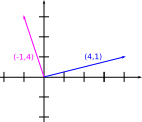
\includegraphics[width = 0.45\linewidth]{3.png}
\end{figure}
\end{minipage}
\item

 \color{pers} Transposing \color{black} a vector is simply converting it from a row-vector to a colum-vector, or a column-vector back to a row-vector.
\[
\vect{1 , 2}^T = \icol{1 \\ 2}
\]

\item \color{groen} Adding \color{black} two vectors is straighforward 
\[
\vect{2 , 1} + \vect{1 , 2} = \vect{3  , 3}
\]

\begin{minipage}{0.45\textwidth}
\begin{flushleft}
Visually, when adding two vectors you simply add one to the end of the other. Note that it does not matter in which order you add them. 
\end{flushleft}
\end{minipage} \hfill
\begin{minipage}{0.45\textwidth}
\begin{figure}[H]
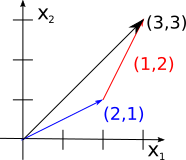
\includegraphics[width = 0.6\linewidth]{1.png}
\end{figure}
\end{minipage}

\item \color{blou} Subtraction\color{black}, like addition, is intuitive
\[
\vect{2 , 1} - \vect{1  , 2} = \vect{1 , -1}
\]

\begin{minipage}{0.45\textwidth}
\begin{flushleft}
Here we negate the vector we are subtracting (the red one in this case) and just like addition we add it to the end of the other. 
	
\end{flushleft}
\end{minipage} \hfill
\begin{minipage}{0.45\textwidth}
\begin{flushleft}
\begin{figure}[H]
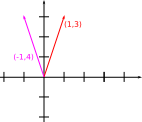
\includegraphics[width = 0.6\linewidth]{2.png}
\end{figure}
\end{flushleft}
\end{minipage}

\end{itemize}

\paragraph{Exercice: } 
Here are 3 vectors, $u = \vect{3 , 5}, v = \vect{8 , 10}, p = \vect{10, 1, 1}$, can you add them together?



\end{document}\begin{beamerboxesrounded}[shadow=true]{}

\end{beamerboxesrounded}